\documentclass[french]{article}
\usepackage[T1]{fontenc}
\usepackage[utf8]{inputenc}
\usepackage{lmodern}
\usepackage[a4paper]{geometry}
\usepackage{babel}
\usepackage{graphicx}

\begin{document}
\title{Nuages de points et modélisation 3D\\
TP 3 : Neighborhood descriptors}
\author{Marius Dufraisse}
\date{}

\maketitle


\paragraph{Question 1.} When the radius is too big small details do not appear in the computed normal map. For instance borders of the windows can be seen when the radius is equal to 50cm (see Figure \ref{fig:q1-50cm}) but when the radius is equal to 5m the wall is in a single color (see Figure \ref{fig:q1-5m}).

When the radius is too small, noise in the data results in noise in the normal (see Figure \ref{fig:q1-5cm} for results with a 5cm radius).



\begin{figure}[h]
	\centering
	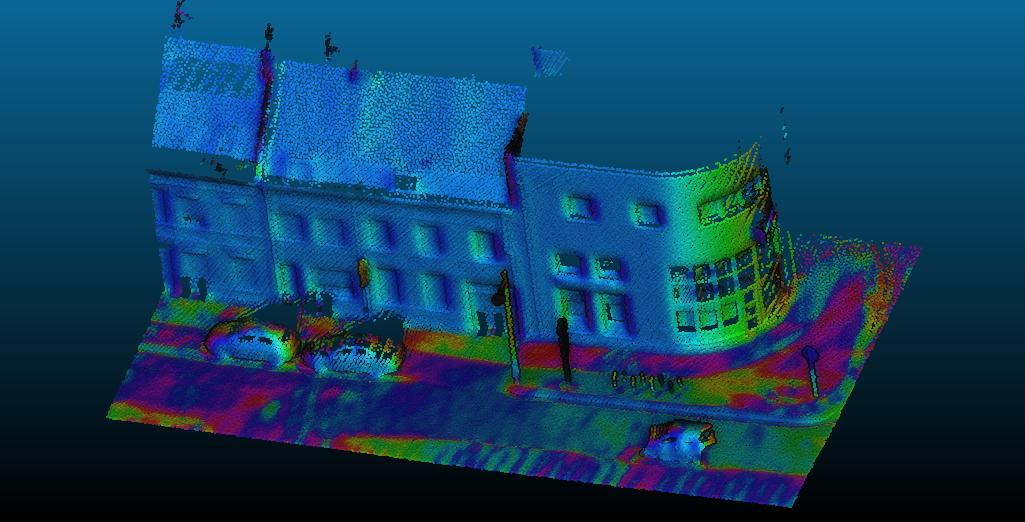
\includegraphics[width=0.6\linewidth]{q1-r50cm.jpg}
	\caption{Normals obtained with a radius of 50cm.}
	\label{fig:q1-50cm}
\end{figure}

\begin{figure}[h]
	\centering
	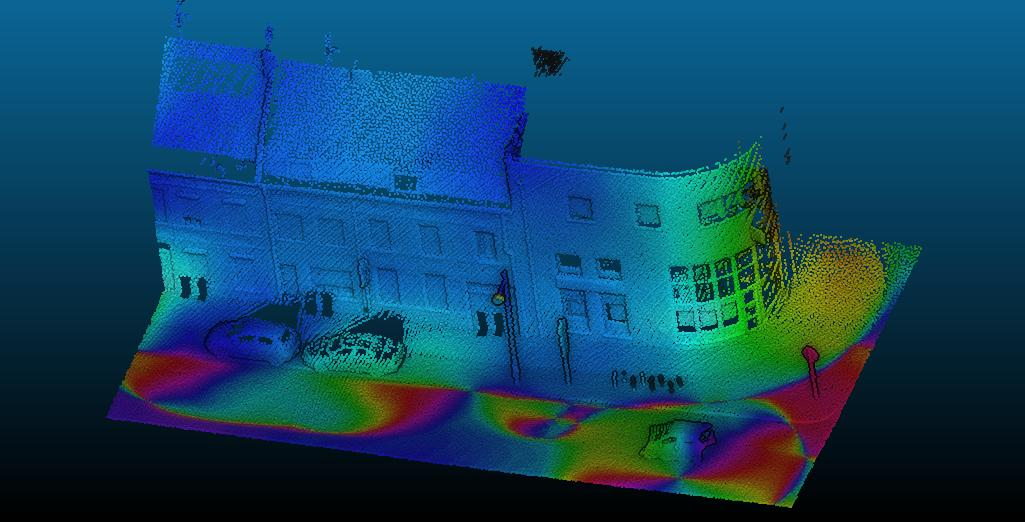
\includegraphics[width=0.6\linewidth]{q1-r5m.jpg}
	\caption{Normals obtained with a radius of 5m.}
	\label{fig:q1-5m}
\end{figure}

\begin{figure}[h]
	\centering
	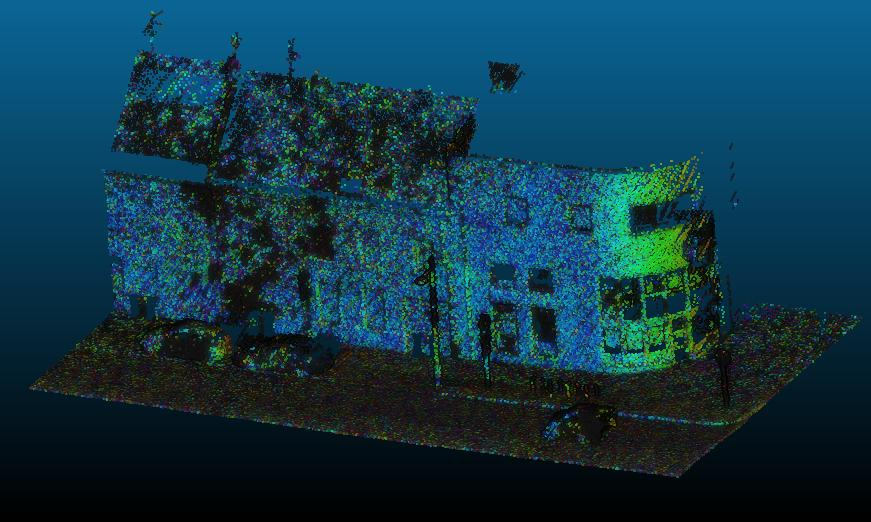
\includegraphics[width=0.6\linewidth]{q1-r5cm.jpg}
	\caption{Normals obtained with a radius of 5cm.}
	\label{fig:q1-5cm}
\end{figure}


\end{document}
